\documentclass[a4paper]{article}
\usepackage[utf8]{inputenc}
\usepackage[T1]{fontenc}
\usepackage[finnish]{babel}
\usepackage{geometry}
\usepackage{amsmath}
\usepackage{amsthm}
\usepackage{amssymb}
\usepackage{graphicx}
\usepackage{multirow}

\theoremstyle{definition}
\newtheorem{lause}{Lause}[section]
\newtheorem{maar}{Määritelmä}
\theoremstyle{remark}
\newtheorem{esim}[lause]{Esimerkki}
\newtheorem*{huom}{Huomautus}

\newcommand{\R}{\mathbb{R}}
\newcommand{\Z}{\mathbb{Z}}
\newcommand{\Q}{\mathbb{Q}}
\newcommand{\N}{\mathbb{N}}
\newcommand{\C}{\mathbb{C}}
\newcommand{\abs}[1]{\left| #1 \right|}

\usepackage{pgf,tikz}
\usetikzlibrary{arrows}
\definecolor{zzttqq}{rgb}{0.6,0.2,0.}
\definecolor{xdxdff}{rgb}{0.490196078431,0.490196078431,1.}
\definecolor{uuuuuu}{rgb}{0.266666666667,0.266666666667,0.266666666667}

\title{\LaTeX -harjoittelua}
\author{Ville Kukkola}
\date{20.3.2015}

\usepackage[colorlinks=true]{hyperref}

\begin{document}

\maketitle

\tableofcontents

\dots

...

Erikoismerkkejä ovat mm. \%, \$ ja \&. Merkkijonon \textbackslash textbackslash tuottaminen onnistuu näin...

% Tämä on kommenttirivi

\section{Liiviläiset}

\subsection{eka}   
Liiviläiset ovat nykyisen Latvian alueella historiallisesti asunut itämerensuomalainen kansa. Liiviläiset muodostivat aikoinaan merkittävän osan Baltian väestöstä, mutta nykyisin he ovat enää pieni kansansirpale. Liiviläisten määrän hupenemiseen vaikuttivat muun muassa latvialaistuminen, Baltiassa riehuneet taudit ja alueella käydyt sodat. 1900-luvulle tultaessa liiviläisiä oli enää eristäytyneellä Kuurinmaan pohjoisrannikolla, jota kutsuttiin myös nimellä Liivinranta. 
\begin{flushright}Vuonna 2010 Latviassa asui \tiny 180 virallisesti rekisteröitynyttä \normalsize liiviläistä.[1] Liiviläisten oma kieli on latvian kielen syrjäyttämä ja \huge äärimmäisen uhanalainen \normalsize : Latvian viimeinen liiviä äidinkielenään puhunut ihminen \emph{kuoli vuonna 2013},[4] mutta kielen myöhemmin opetelleita on \underline{jonkin verran}. Liiviläinen kulttuuri ja kieli ovat latvialaisten niitä kohtaan kokeman mielenkiinnon takia hiljattain kokeneet uuden nousukauden.
\end{flushright}

Vaihdannaisessa renkaassa pätee \((a+b)^2=a^2+2ab+b^2\). Jos siis \(2ab=0\), niin $(a+b)^2 \neq a^2 + b^2$.
Funktion $f:\mathbb{R}\rightarrow\mathbb{R}$ derivaatta pisteessä $x_0\in\mathbb{R}$ on
\[
f'=\lim_{x \rightarrow x_0}\frac{f(x)-f(x_0)}{x-x_0}
\]
mikäli raja-arvo on olemassa.

Jos $F$ on $\sigma$ -algebra ja \(A_i\in F\) kaikilla $i=1,2,\dots ,$ niin
\[
\bigcup_{i=1}^\infty A_i\in F
\]
Vektoreiden $\overline{v} = \overline{AB}$ ja $\overline{w} = \overline{CB}$ ristitulo $ \overline{v} \times \overline{w}$ on kohtisuorassa kumpaakin vektoria vastaan. Pistetulo \( \overline{v} \cdotp{} \overline{w} \) on sen sijaan reaaliluku.

\subsection*{toka}
Liiviläisiä tai heidän jälkeläisiään asuu myös Latvian ulkopuolella. Joidenkin lähteiden mukaan liiviläisten perinteiset asuinalueet olisivat ulottuneet Etelä-Viroon saakka. Maailmansotien aikana monet liiviläiset muuttivat pakolaisiksi Ruotsiin, josta osa jatkoi etenkin Kanadaan ja Yhdysvaltoihin. Viimeinen liiviä äidinkielenään puhunut henkilö elikin Kanadassa, mutta hän kuoli vuonna 2013.[5]


\section{Tutkimus}

1200-luvulta peräisin oleva Henrikin Liivinmaan kronikka on yksi tärkeimmistä liiviläisistä kertovista historiallisista lähteistä. Sen jälkeen kului 350 vuotta ennen kuin liiviläisistä julkaistiin merkittävää kirjallisuutta. Thomas Hiärne (1638–1678) käsitteli Kuurin- ja Liivinmaan liiviläisiä omassa Liivinmaan kronikassaan. Parikymmentä vuotta Hiärnen kuoleman jälkeen ilmestyivät P. Einhornin Historia Lettica ja A. L. Schlözerin tutkimus liiviläisistä. August Wilhelm Hupel (1737–1819) kertoi teoksissaan liiviläisistä sekä liivin kielestä ja korosti kansan ja kielen yhteyttä muihin itämerensuomalaisiin kansoihin ja kieliin. Heinrich von Jannau (1753–1821) tutki Salatsin alueen liiviläismurteen ja viron kielen yhteyksiä ja piti liiviläisiä alkuvirolaisina, minkä useat tutkijat myöhemmin todistivat vääräksi. Anders Johan Sjögren teki Latviaan tutkimusmatkoja vuosina 1846 ja 1852 Venäjän maantieteellisen seuran kehotuksesta ja tutki liivin itä- ja länsimurteen puhujia. Sjögrenin kuoltua työtä jatkoi hänen keräämänsä aineiston pohjalta Ferdinand Johan Wiedemann. Wiedemann julkaisi vuonna 1861 suurteoksen Joh. Andreas Sjögren's Livische Grammatik nebst Sprachproben, joka teki liivin tunnetuksi yhtenä itämerensuomalaisista kielistä. Wiedemannin jälkeen liiviläisiä tutki Eemil Nestor Setälä, joka kokosi liiviläisiä kertomuksia, sananlaskuja ja kansanlauluja.[6]

\[
\{ 2^n|n \in \mathbb{Z} \} = \left\lbrace \left( \frac{1}{2} \right) ^n \middle| n  \in \mathbb{Z} \right\rbrace
\]
\begin{lause}
Jos $F$ on $\sigma$-algebra ja $P:F \rightarrow \mathtt{R}$ todennäköisyys, niin tapahtumille $A_1, A_2, \dots \in F$ pätee
\[
P \left( \bigcup_{i=1}^\infty A_i \right) \leq \sum _{i=1}^\infty P \left( A \right)
\]
\end{lause}
\begin{proof}
Seuraa todennäköisyyden ja $\sigma$-algebran määrittelmistä. Todistus jätetään harjoitustehtäväksi.
\end{proof}
\begin{esim}
Laskutoimitusten ominaisuuksien nojalla
\begin{align*}
(a+b)(c+d) &= a(c+d)+b(c+d)\\
		&=ac+ad+bc+bd\\
		&=c(a+b)+d(a+b)\\
		&=(c+d)(a+b)\\	
\end{align*}

\begin{multline*}
(a+b)(c+d)=a(c+d)+b(c+d)
=ac+ad+bc+bd
=c(a+b)+d(a+b)\\
=(c+d)(a+b)=c(a+b)+d(a+b)=ac+ad+bc+bd=a(c+d)+b(c+d)=(a+b)(c+d
\end{multline*}
\end{esim}

\begin{maar}
Eksponenttifunktiolla on sarjakehitelmä
\begin{equation}\label{expsarja}
e^x= \sum_{n=1}^\infty \frac{x^n}{n!}
\end{equation}
\end{maar}

\begin{maar}
Funktion $f:\mathbb{R}\rightarrow\mathbb{R}$ derivaatta pisteessä $x_0\in\mathbb{R}$ on
\[
f'=\lim_{x \rightarrow x_0}\frac{f(x)-f(x_0)}{x-x_0}
\]
mikäli raja-arvo on olemassa.
\end{maar}


1900-luvun alun tärkeimpiä liiviläisten tutkijoita olivat Lauri Kettunen ja Oskar Loorits, jotka julkaisivat useita teoksia liiviläisistä ja liivin kielestä. Tutkimuksen lisäksi he halusivat kohottaa liiviläisten kansallistunnetta ja tukivat paikallisia kansallisia hankkeita. Kansallisaatteen nousun myötä tutkimusta alkoivat harjoittaa myös liiviläiset itse, kuten esimerkiksi kieltä tutkinut Petõr Damberg.[7] Toisen maailmansodan aikana tutkimus keskeytyi, mutta sodan jälkeen Tarton yliopiston tutkijat jatkoivat sitä. Neuvostovallan aikaan Liivinrannalle pääsyyn tarvittiin erikoislupa ja se myönnettiin Tarton yliopistolle helpommin kuin muille. Tänä aikana tutkimuksia tekivät eritoten Paul Ariste ja Eduard Vääri.[8] Vuonna 2005 kuollutta Eduard Vääriä on pidetty Viron merkittävimpänä liivin kielen ja liiviläisyyden asiantuntijana.[9]
Historia


\begin{huom}
Laskareissa kannattaa muistaa eksponenttifunktion sarjakehitelmä \eqref{expsarja} \pageref{expsarja}.
\end{huom}

\begin{enumerate}
\item käy luennolla
\item palaute laskarit
\item käy kaupassa, Osta:	
	\begin{itemize}
		\item maitoa
		\item leipää
		\item viiliä
		\item tuliaiset
		\begin{itemize}
			\item kaljaa
			\item sipsiä
			\item dippiä
		\end{itemize}
	\end{itemize}
\end{enumerate}

Matemaatikoita:
\begin{description}
	\item[Euler]
	\item[Gauss]
	\item[Bolzano]
\end{description}

Lukujoukot muodostavat tornin
\[
\N \subset \Z \subset \Q \subset \R \subset \C .
\] \[
\Z \not\subset \N
\]

\[
\abs{\abs{x} - \abs{y}} \leq \abs{x+y} \leq \abs{x} + \abs{y}
\] ja \[
\abs{\int_a^b f(x)dx} \leq \int_a^b \abs{f(x)} dx .
\]

\section{esihistoria}


\includegraphics[scale=1.5]{OldGuy}

Liiviläisten esi-isien uskotaan tulleen asuinalueilleen Väinäjokea pitkin.[10][11] Rautakaudella ja keskiajalla liiviläiset asuttivat laajaa aluetta Latvian keski- ja pohjoisosista Väinä- ja Gaujajokien varsilla Vidzemen alueella. Myös Kuurinmaan pohjoiskärjessä asunut itämerensuomalainen väestö on myöhemmin yhdistetty liiviläisiin, vaikka vielä keskiajalla näin ei tehty. Kuurinmaan liiviläisestä väestöstä käytettiin nimitystä kuurit, jolla viitataan myös balttilaiseen kuurien heimoon; nimitystä käytettiin yleisesti kaikista Kuurinmaan asukkaista.  Liiviläisten merkitystä heijastaa se, että koko Liivinmaa nimettiin keskiajalla heidän mukaansa.[10]
Kivikausi
\begin{figure} [pbt]
	
\includegraphics[scale=1.5]{OldGuy}
	\caption{Toimii!}
	\label{harold}
\end{figure}
Baltian alueella on liikkunut ihmisiä tiettävästi jo 13 000 vuotta sitten. DNA-tutkimukseen perustuvan, erittäin kiistellyn teorian mukaan alueella liikkui uralilaisia kieliä puhuvia kansoja jo 10 000 vuotta sitten.[12] Osa tutkijoista katsoo, että uralilaista (suomalais-ugrilaista) kieltä puhuttiin Itämeren alueella aikaisintaan pronssikaudella.[13] Alueen ensimmäiset asukkaat kuuluivat niin sanottuun peuranmetsästäjien kulttuuriin. He metsästivät peuroja ja muuttivat etelän ja pohjoisen välillä peurojen muuttoliikkeen mukaan. Peurat hävisivät Baltian alueelta noin 7500 eaa. Alueelta on löydetty vuosilta 4000–1500 eaa. peräisin olevaa neoliittiselle kivikaudelle tyypillistä keramiikkaa. Vuosina 2000–1500 eaa. alueelle levisi nuorakeraaminen kulttuuri, joka tunnetaan myös nimellä vasarakirveskulttuuri. Se sai nimensä tuon ajan hautauksista löydetyistä vasaran muotoisista kirveistä. Kuurinmaalla oli havaittavissa kaksi eri kulttuuria, etelässä indoeurooppalaisena pidetty nuorakeraaminen ja pohjoisessa kampakeraaminen kulttuuri, jota on usein pidetty suomalais-ugrilaisena.[14]
Pronssikausi



fdasfdsafdsafdsafdsafdafdas


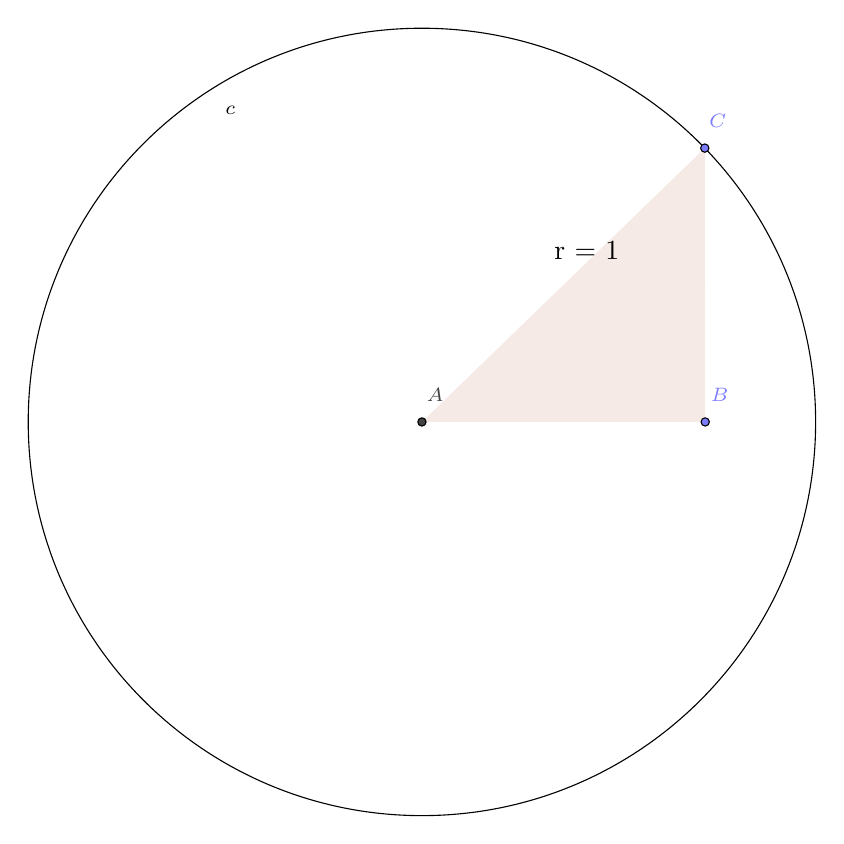
\begin{tikzpicture}[line cap=round,line join=round,>=triangle 45,x=5.0cm,y=5.0cm]
\fill[color=zzttqq,fill=zzttqq,fill opacity=0.1] (0.,0.) -- (0.719517336606,0.) -- (0.718495771734,0.695531326398) -- cycle;
\draw (0.,0.) node [anchor = north] (r=1) {};
\draw(0.,0.) circle (5.cm);
\draw (0.31183722768,0.482821945672) node[anchor=north west] {r = 1};
\begin{scriptsize}
\draw [fill=uuuuuu] (0.,0.) circle (1.5pt);
\draw[color=uuuuuu] (0.0338591380444,0.0683818847612) node {$A$};
\draw[color=black] (-0.486718011636,0.791124917813) node {$c$};
\draw [fill=xdxdff] (0.719517336606,0.) circle (1.5pt);
\draw[color=xdxdff] (0.756602171096,0.0683818847612) node {$B$};
\draw [fill=xdxdff] (0.718495771734,0.695531326398) circle (1.5pt);
\draw[color=xdxdff] (0.751548024012,0.765854182392) node {$C$};
\end{scriptsize}
\end{tikzpicture}

\begin{figure} [ht]
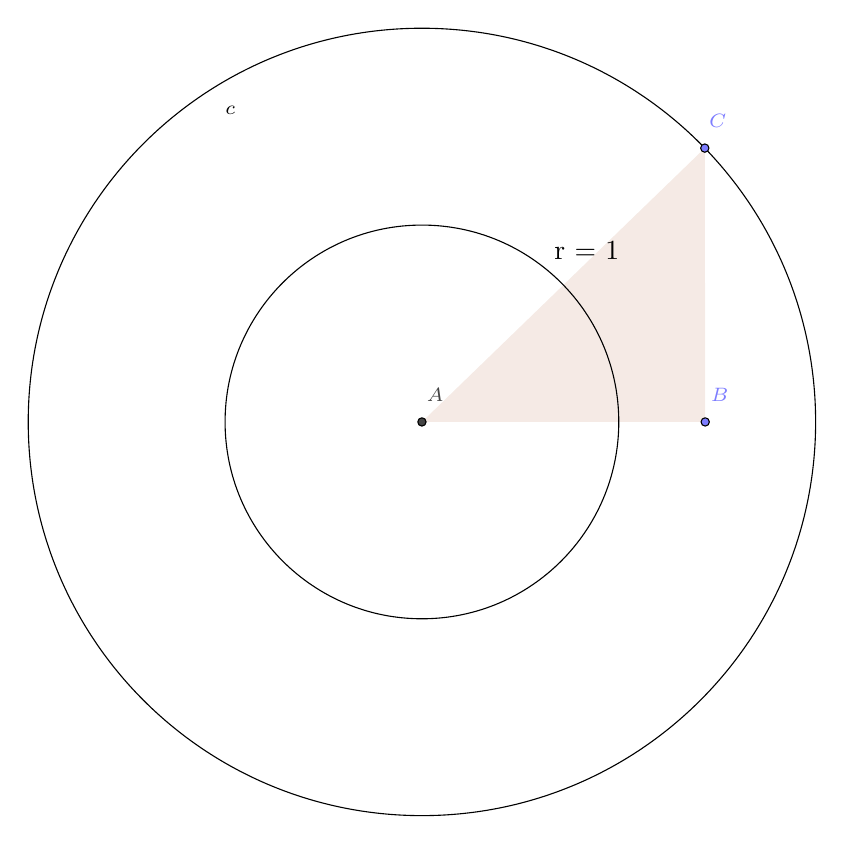
\begin{tikzpicture}[line cap=round,line join=round,>=triangle 45,x=5.0cm,y=5.0cm]
\fill[color=zzttqq,fill=zzttqq,fill opacity=0.1] (0.,0.) -- (0.719517336606,0.) -- (0.718495771734,0.695531326398) -- cycle;
\draw (0.,0.) node [anchor = north] (r=1) {};
\draw(0.,0.) circle (5.cm);
\draw(0.,0.) circle (2.5cm);
\draw (0.31183722768,0.482821945672) node[anchor=north west] {r = 1};
\begin{scriptsize}
\draw [fill=uuuuuu] (0.,0.) circle (1.5pt);
\draw[color=uuuuuu] (0.0338591380444,0.0683818847612) node {$A$};
\draw[color=black] (-0.486718011636,0.791124917813) node {$c$};
\draw [fill=xdxdff] (0.719517336606,0.) circle (1.5pt);
\draw[color=xdxdff] (0.756602171096,0.0683818847612) node {$B$};
\draw [fill=xdxdff] (0.718495771734,0.695531326398) circle (1.5pt);
\draw[color=xdxdff] (0.751548024012,0.765854182392) node {$C$};
\end{scriptsize}
\end{tikzpicture}
\caption{pienempi ympyrä}
\end{figure}

Vuoden 1500 eaa. tienoilla alueelle alkoi saapua pronssisia tarve-esineitä ja koruja. Tällöin Väinäjoki erotti selvästi kaksi kulttuuriryhmittymää toisistaan. Pronssilöydökset Väinäjoen eteläpuolelta ovat runsaammat, sillä eteläosat saivat helposti pronssia vaihtamalla sitä meripihkaan, jota saatiin meripihkarannikolta. Vuosina 1000–600 eaa. Väinäjoen pohjoispuolelle syntyi uusi kulttuuri – erään teorian mukaan kyse oli uudesta suomalais-ugrilaisesta muuttoaallosta alueelle. Liivinmaan tuon ajan kansojen sijoittumisesta on vaikeaa saada tarkkaa tietoa, mutta yhtenä keinona on käytetty hautaustapojen tutkimusta. Pronssikaudella Etelä-Virossa ja Väinäjoen pohjoispuolella hautaukset tehtiin pääasiallisesti pohjois-eteläsuunnassa, kun taas Väinäjoen eteläpuolella ne tehtiin itä-länsisuunnassa.[15] Pronssikaudella yleistyi myös vainajien polttohautaus. Kuitenkin etenkin sisämaassa vainajat haudattiin vielä pitkään maahan.[16]
Rautakausi

\begin{tabular}{r|cc}
Joukkue & pisteet & ottelut \\
Barcelona & 9 & 3 \\
Arsenal & 6 & 3 \\
PSV & 1 & 2 \\
Basel & 1 & 2\\
\end{tabular}

\begin{tabular}{r||c|c}
Joukkue & pisteet & ottelut \\
\hline
Barcelona & 9 & 3 \\
Arsenal & 6 & 3 \\ \cline{2-3}
PSV & 1 & 2 \\ 
Basel & 1 & 2\\
\end{tabular}

\begin{tabular}{|c|c|c|}
\hline
\multicolumn{3}{|c|}{\textbf{Päiväpetolintuja}} \\
\hline
\textit{Nimitys} &\textit{Suku} &\textit{Laji} \\
\hline
Kanahaukka & Accipiter & gentilis \\
Hiirihaukka & Buteo & buteo \\
Tuulihaukka & Falco & columbarius \\
Nuolihaukka & Falco & subbuteo \\
\hline
\end{tabular}



%Tehtävä 3.8 ja 9: Sijoitetaan taulukko tasan tähän, mikäli mahdollista, jotta se on helppo löytää koodin tuloksen tarkastamiseksi
\begin{table} [htb]
\title{Haukat}
\begin{tabular}{|c|c|c|c|}
\hline
\textit{Heimo} &\textit{Nimitys} &\textit{Suku} &\textit{Laji} \\
\hline
\multirow{2}{*}{Haukat} &Kanahaukka & Accipiter & gentilis \\
\cline{2-4} & Hiirihaukka & Buteo & buteo \\
\hline
\end{tabular}
\caption{Kana- ja hiirihaukka ovat haukkoja.}
\label{haukat}
\end{table}

% Ei sulkuja
\[
\begin{matrix}
1 & 2 & 3 \\
4 & 5 & 6 \\
\end{matrix}
\]

% Hakasulkeet
\[
\begin{bmatrix}
1 & 2 & 3 \\
4 & 5 & 6 \\
\end{bmatrix}
\]

%pystyviivat, determinantti
\[
\begin{vmatrix}
1 & 2 & 3 \\
4 & 5 & 6 \\
\end{vmatrix}
\]
%%%%%%%%%%%%%%%%%%%%%
\[
\begin{bmatrix}
0 & 0 & 1 & a_1 \\
0 & 1 & 1 & a_2 \\
1 & 1 & 1 & a_3
\end{bmatrix}
\xrightarrow{R_1 \leftrightarrow R_2} 
\begin{bmatrix}
1 & 1 & 1 & a_3 \\
0 & 1 & 1 & a_2 \\
0 & 0 & 1 & a_1
\end{bmatrix}
\]


\section{Rautakausi}

Rautakausi alkoi alueella 600–500 eaa. Ensimmäiset maininnat fenni- ja levonikansoista esiintyivät 100-luvulla Tacituksen ja Ptolemaioksen teoksissa. Ne eivät kuitenkaan liene viitanneet nykyisiin suomalaisiin tai liiviläisiin kansoihin. 500–600-luvuilla slaavit alkoivat työntyä silloisten itäbalttien alueelle ja baltit alkoivat siirtyä pohjoiseen: kuureja muutti pohjoisempaan Kuurinmaahan, seelit muuttivat syvemmälle nykyiseen Seloniaan ja latgallit muuttivat pidemmälle nykyiseen Latgaleen. 500 eaa.–700 jaa. alueella käytettiin kiviarkkuhautoja ja vainajat mahdollisesti poltettiin. Väinäjoki oli tärkeä kauppareitti, ja sen varrelta on useita bysanttilaisia ja saksalaisia rahalöytöjä. Viikingit tekivät retkiä Baltiaan ja verottivat sen asukkaita 700–1000-luvuilla. He eivät kuitenkaan koskaan vakiinnuttaneet asemaansa, vaikka heillä oli alueella lyhytaikaisia tukikohtia.
% t. 4.1 ja 2
Alueella tavataan erilaisia haukkoja ks. taulukko \ref{haukat} sivulla \pageref{haukat}. Otapa huikka kahvia kuten kuvan \ref{harold} kaveri sivulla \pageref{harold}.
\begin{quote}
''Viekas kettu punaturkki laiskan koiran takaa kurkki. Viekas kettu punaturkki laiskan koiran takaa kurkki\dots ''
\begin{flushright}
--Microsoft Word
\end{flushright}
\end{quote}

\begin{verse}
Out spake the brave Horatius\\
the Captain of the Gate:\\
''To every man upon this Earth\\
death cometh soon or late.\\
And how can a man die better \\
than facing fearful odds, \\
for ashes of his fathers,\\
and temples of his gods''
\end{verse}

Viimeistään 1000-luvulla\footnote{tai aiemmin} Baltian heimot järjestäytyivät muinaismaakunniksi, ja liiviläisten asuinalueet olivat vakiintuneet 1100-luvun alkuun mennessä. Liiviläisiä muinaismaakuntia olivat Liivinmaalla Livones Veinalenses, Idumeja, Metsepole ja Toreida sekä Kuurinmaalla Venema ja Ventava.Pohjoisessa liiviläisten alueen on arvioitu rajoittuneen Salatsijoelle, idässä Lielvarden–Aizkrauklen linjalle ja etelässä Väinäjoelle. Pohjoisessa heidän naapureinaan olivat virolaiset, etelässä semgallit ja seelit ja idässä latgallit. Kuurinmaalla liiviläisiä asui Riianlahden itärannalla Kuurinmaan pohjoiskärkeen saakka ja sieltä edelleen Ventspilsin ja Liepajan puoliväliin saakka 40–50 km:n syvyydessä sisämaahan. Hajanaisemmin heitä asui Itämeren rannalla aina Memelin seuduille saakka. 1100-luvulla tanskalainen arkkipiispa Absalon kävi kastamassa kuureja ja rakensi Kuurinmaan pohjoiskärkeen kirkon, mutta käännytettyjen määrä oli luultavasti hyvin pieni. Nykyisin paikalla on Kolkan kylä, jonka liivinkielisen nimityksen Kuolka arvellaan tarkoittavan samaa kuin suomen sana kolkka. 1000-luvulta peräisin olevassa Adam Bremeniläisen kronikassa mainitaan Eesti, Kuurinmaa, vepsäläiset ja merjalaiset mutta ei liiviläisiä. 1100-luvulla Nestorin kronikassa mainitaan suomensukuinen heimo nimeltä libj, Henrik Lättiläinen taas käytti Liivinmaan kronikassa liiviläisistä nimitystä livones. Sama nimi mainitaan teoksessa Livonian kaikuja 1290-luvulta.

Joukko on suljettu jos sen komplementti on avoin. \cite{topo1} Kompleksiluvut $\C$ muodostavat kunnan. \cite{rudin} Jotakin algebrasta \cite{kemper}


\bibliographystyle{plain}
\bibliography{lahteet,Rudin}

\end{document}
